\apendice{Plan de Proyecto Software}

\section{Introducción}
La planificación de un proyecto es esencial para su éxito, ya que nos permite ver cuales van a ser las necesidades, los impedimentos y otra serie de eventos o circunstancias relevantes en el desarrollo del proyecto. La planificación de un proyecto software tiene diversas partes que tratan temas como la planificación temporal o el uso de licencias.

La planificación de este proyecto se ha divido en dos secciones:
\begin{itemize}
	\item \textbf{Planificación temporal:} Sección donde se puede ver la distribución temporal del proyecto, dividido en \textit{sprints}. Cada \textit{sprint} está formado por una serie de tareas relacionadas con una estimación individual de tiempo. 
	\item \textbf{Estudio de viabilidad:} Sección orientada a la viabilidad del proyecto, es decir, cuando favorable es su realización, en aspectos económicos y legales.
	\begin{itemize}
		\item \textbf{Viabilidad económica:} En esta subsección comentaré los gastos que ha tenido el desarrollo del proyecto.
		\item \textbf{Viabilidad legal:} Subsección en la que expondré las distintas licencias de las librerías que han sido necesarias para el desarrollo del proyecto y la licencia final del producto.
	\end{itemize}
\end{itemize}

En este proyecto he seguido, además, la metodología \textit{SCRUM} gracias a la \textit{GitHub} junto con \textit{ZenHub}, pudiendo así hacer una planificación correcta y desarrollo incremental.
\section{Planificación temporal}
En esta sección voy a comentar el desarrollo temporal del proyecto divido en distintos \textit{sprints}, por cada uno de ellos voy a comentar:
\begin{itemize}
	\item Fecha de inicio y de cierre del \textit{sprint}.
	\item Pequeña descripción de lo que se pretendía hacer en el \textit{sprint}.
	\item Lista agrupando y resumiendo las tareas correspondientes.
	\item Gráfico \textit{Burndown} que nos permite ver el desarrollo del \textit{sprint}, estos gráficos en los primeros \textit{sprints} no se ve un progreso claro, debido a que no se ha bien el gráfico al haber estado el repositorio en modo privado, hasta el \textit{sprint} 11.
	\item Breve comentario sobre el desarrollo del \textit{sprint}.
\end{itemize}

\subsection{Sprint 1}
Este \textit{sprint} se inició el 4 de Diciembre de 2018 y se cerró el 22 de Febrero de 2019.

En este \textit{sprint}, que al final por como sucedieron las cosas se alargó al no saber cuando podría cerrarlo, se orientó a la creación del repositorio en Git, a la creación del documento donde poder apuntar los aspectos más relevantes de la investigación junto con el investigador colaborardor, Sergio Chico, también se quería empezar con las tareas de investigación y las primeras reuniones con APACE Burgos.

La lista resumen de las tareas que se realizaron en este \textit{sprint} 1 son:
\begin{itemize}
	\item Investigación de la clasificación de audios.
	\item Aprender a desarrollar una aplicación de \textit{Android}.
	\item Aprender a desarrollar una aplicación \textit{Android} que permita grabar~\cite{record}.
	\item Implementación del primer prototipo de grabación de audios.
	\item Investigación y documentación del estudio sobre el audio en \textit{Android} y \textit{MediaRecorder}.
	\item Continuas reuniones y visitas con APACE Burgos para determinar los objetivos y funcionalidades del proyecto.
\end{itemize}

Al ser el primer \textit{sprint} es el más desordenado, tuve en su momento un problema, ya que no sabía exactamente cuando parar y cerrar el \textit{sprint}. Aun así, fue un \textit{sprint} importante donde se definieron los primeros objetivos y funcionalidades, y sirvió para conocer que querían desde APACE.

\subsection{Sprint 2}
Este \textit{sprint} comenzó el 22 de Febrero de 2019 y terminó el 25 de Febrero de 2019.

En este \textit{sprint} se quería diseñar la interfaz de la aplicación de generación de datos, además de crear las pantallas a partir de la interfaz diseñada y crear su estructura.

La lista resumen de las tareas del \textit{sprint} 2 es:
\begin{itemize}
	\item Aprender a crear varias pantallas en una aplicación \textit{Android}.
	\item Diseño con \textit{Pencil} de la interfaz de la aplicación para generar los datos a partir de la información de las reuniones.
	\item Crear las pantallas según el diseño.
\end{itemize}

\begin{figure}
	\centering
	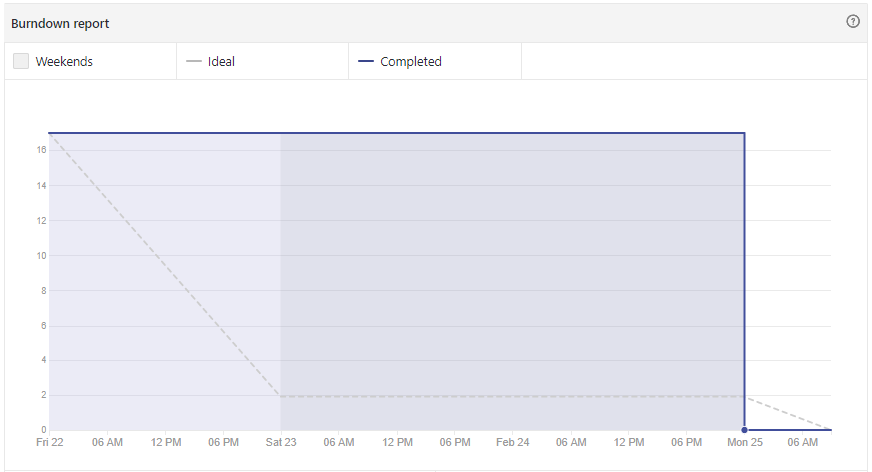
\includegraphics[width=\textwidth]{sprint2}
	\caption{Gráfico del desarrollo del \textit{sprint} 2.}
	\label{fig:sprint2}
\end{figure}

En este \textit{sprint}~\ref{fig:sprint2} se cometió el error contrario al anterior, este \textit{sprint} quizás sea demasiado corto, aun así se siguió correctamente la planificación inicial.

\subsection{Sprint 3}
Este \textit{sprint} empezó el 25 de Febrero de 2019 y acabó el 7 de Marzo de 2019.

En este \textit{sprint} se quería implementar las funcionalidades de las diferentes pantallas, además de implementar la navegabilidad entre estas.

Las tareas que se realizaron en este \textit{sprint} se resumen en:
\begin{itemize}
	\item Crear las funcionalidades de las distintas pantallas.
	\item Implementar la navegabilidad entre pantallas.
	\item Corrección de \textit{bugs}.
	\item Implementar la generación de comprimidos.
	\item Comentar el código.
\end{itemize}

\begin{figure}
	\centering
	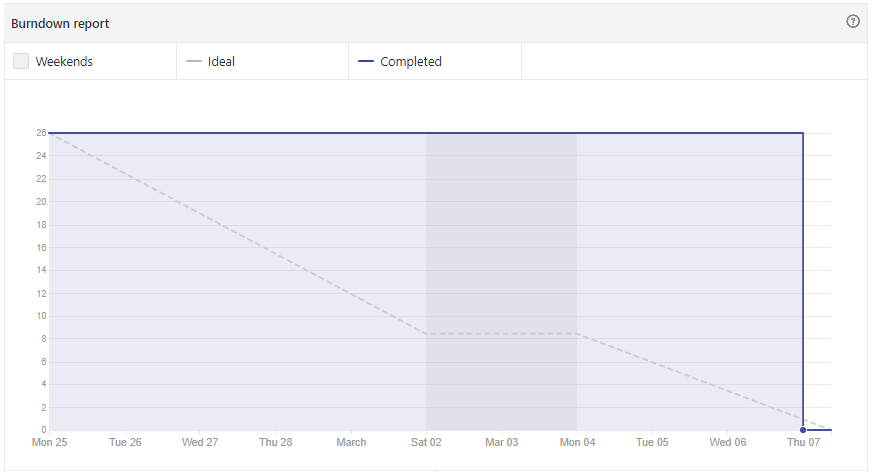
\includegraphics[width=\textwidth]{sprint3}
	\caption{Gráfico del desarrollo del \textit{sprint} 3.}
	\label{fig:sprint3}
\end{figure}

En este \textit{sprint}~\ref{fig:sprint3}, como en el anterior, se consigue correctamente los objetivos en el tiempo que se quería. Esto era esencial, ya que necesitábamos tener la aplicación que nos permitía generar datos lo antes posible, para contar con el mayor número de ellos al final del proyecto.

\subsection{Sprint 4}
Este \textit{sprint} comenzó el 7 de Marzo de 2019 y terminó el 18 de Marzo de 2019.

En este \textit{sprint} se quería implementar el método de envío de los comprimidos desde la aplicación según se definiese en la reunión. Y complementar la aplicación con las emociones y las opciones adicionales que nos tenía que facilitar APACE.

Las tareas que se realizaron en este \textit{sprint} 4 son:
\begin{itemize}
	\item Resumir las opciones adicionales facilitadas por APACE.
	\item Modificación de las pantallas de Estado y de Opciones con los nuevos valores.
	\item Implementación del envío de los comprimidos por correo.
	\item Creación del manual de usuario de la aplicación.
	\item Crear la presentación en \textit{Power Point} para enseñar la aplicación.
	\item Presentación ante familias y cuidadores de la aplicación.
\end{itemize}

\begin{figure}
	\centering
	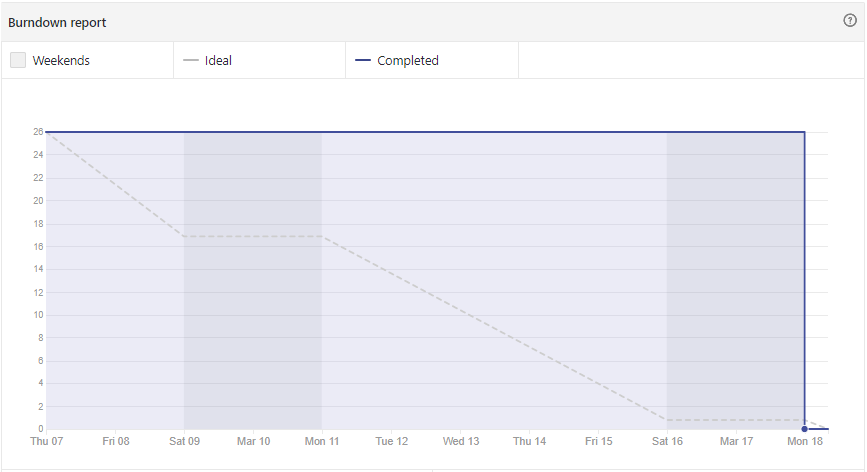
\includegraphics[width=\textwidth]{sprint4}
	\caption{Gráfico del desarrollo del \textit{sprint} 4.}
	\label{fig:sprint4}
\end{figure}

En este \textit{sprint} 4~\ref{fig:sprint4} se ha realizado más tareas de las que se pretendía en un principio, ya que no se contaba con tener que hacer la presentación en APACE para mostrar y ayudar a instalar la aplicación.

\subsection{Sprint 5}
Este \textit{sprint} comenzó el 18 de Marzo de 2019 y acabó el 5 de Abril de 2019.

En este \textit{sprint} se pretendía realizar el diseño de la interfaz de la aplicación de interpretación, y generar mis propios datos con la aplicación de generación de datos, ya que como se comentó en la reunión, lo más seguro es que no tuviésemos suficientes datos.

Las tareas del \textit{sprint} 5 se pueden resumir en:
\begin{itemize}
	\item Presentación de la aplicación de generación de datos a las familias que no pudieron estar en la anterior presentación.
	\item Diseño de las posibles interfaces de la aplicación de interpretación.
	\item Diseño de la aplicación.
	\item Elección junto con APACE de la interfaz final.
	\item Generación de mis propios datos.
\end{itemize}

\begin{figure}
	\centering
	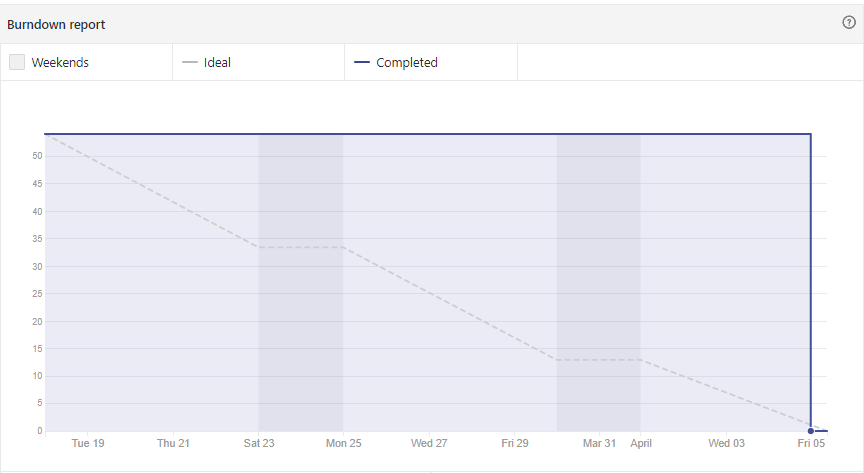
\includegraphics[width=\textwidth]{sprint5}
	\caption{Gráfico del desarrollo del \textit{sprint} 5.}
	\label{fig:sprint5}
\end{figure}

Este \textit{sprint} 5~\ref{fig:sprint5} costó mucho, ya que la grabación de audios se hizo muy larga, ya que debía de ser precisa. Aun así el \textit{sprint} transcurrió correctamente.

\subsection{Sprint 6}
Este \textit{sprint} comenzó el 5 de Abril de 2019 y terminó el 11 de Abril de 2019.

En este \textit{sprint} se quería, a partir de los diseños hechos en el \textit{sprint} anterior, crear e implementar las funcionalidades de la aplicación de interpretación.

Las tareas que se realizaron en este \textit{sprint} son:
\begin{itemize}
	\item Crear las pantallas y las clases diseñadas.
	\item Implementar las funcionalidades de las clases.
	\item Implementar la navegabilidad entre pantallas.
	\item Modificar las imágenes pasadas por APACE para la accesibilidad.
	\item Implementar el paciente por defecto.
\end{itemize}

\begin{figure}
	\centering
	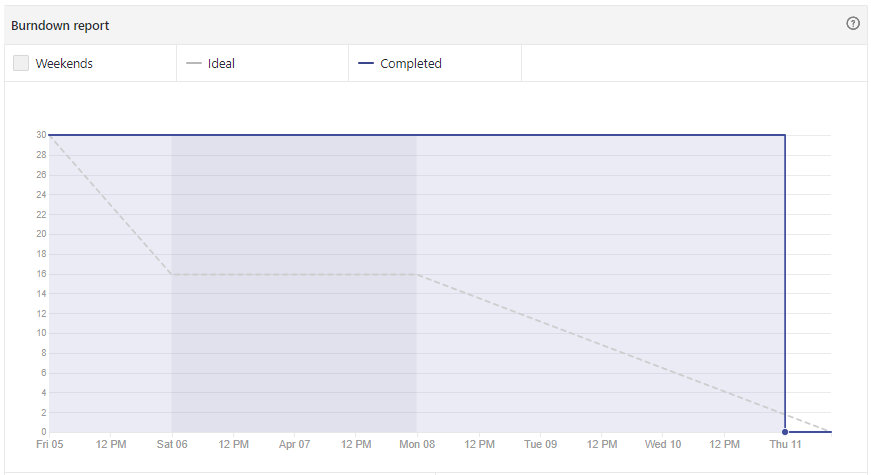
\includegraphics[width=\textwidth]{sprint6}
	\caption{Gráfico del desarrollo del \textit{sprint} 6.}
	\label{fig:sprint6}
\end{figure}

En el \textit{sprint} 6~\ref{fig:sprint6} se ha seguido correctamente la idea inicial de los objetivos marcados para este.

\subsection{Sprint 7}
Este \textit{sprint} va desde el día 11 de Abril de 2019 hasta el día 28 de Abril de 2019.

En el séptimo \textit{sprint} se quería diseñar e implementar diferentes tipos de test que permitan probar las distintas partes de la aplicación, y corregir los \textit{bugs} resultantes.

El resumen de las tareas de este \textit{sprint} es:
\begin{itemize}
	\item Diseño de los test unitarios.
	\item Implementación de los test unitarios.
	\item Diseño de los test de integración.
	\item Implementar los test de integración.
	\item Realizar el \textit{Monkey test}.
	\item Comentar el código de los test.
	\item Corrección de los \textit{bugs} detectados.
\end{itemize}

\begin{figure}
	\centering
	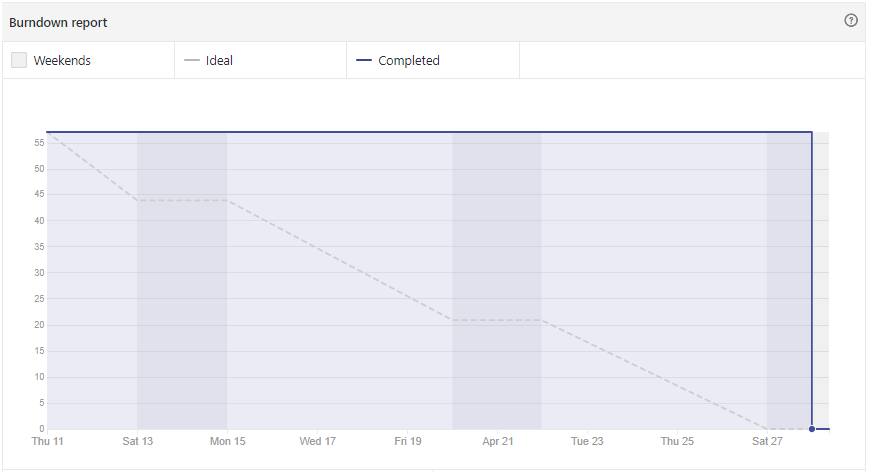
\includegraphics[width=\textwidth]{sprint7}
	\caption{Gráfico del desarrollo del \textit{sprint} 7.}
	\label{fig:sprint7}
\end{figure}

Este ha sido uno de los \textit{sprints} más costosos y a la vez más favorables para el proyecto~\ref{fig:sprint7}, ya que aunque llevó mucho tiempo diseñar e implementar todos los test dio como resultado encontrar algunos \textit{bugs} que no podría haber detectado de otra manera.

\subsection{Sprint 8}
Este \textit{sprint} se desarrolló desde el 28 de Abril de 2019 hasta el 10 de Mayo de 2019.

En este \textit{sprint} se quería modificar las cosas que nos comentó APACE sobre la interfaz, añadir la pantalla de información y sus test correspondientes, y por último comenzar con el diseño del servidor.

Las tareas que finalmente se hicieron fueron:
\begin{itemize}
	\item Cambios en la interfaz pedidos por APACE.
	\item Implementación de la pantalla de información.
	\item Cambios en los diseño, para añadir la nueva información.
	\item Diseño de los test para la pantalla de información.
	\item Implementación de los test de la pantalla de información.
	\item Diseñar el servidor.
	\item Implementar el servidor.
	\item Probar la implementación del servidor.
\end{itemize}

\begin{figure}
	\centering
	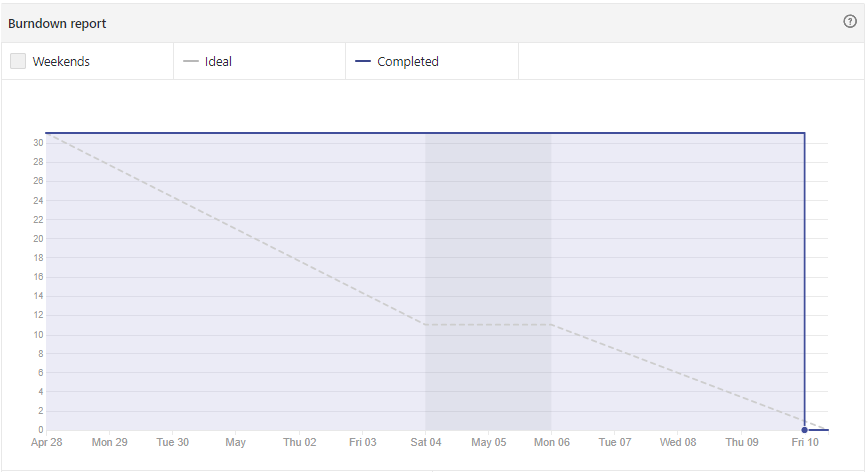
\includegraphics[width=\textwidth]{sprint8}
	\caption{Gráfico del desarrollo del \textit{sprint} 8.}
	\label{fig:sprint8}
\end{figure}

En este \textit{sprint} 8~\ref{fig:sprint8} al final se realizaron todas la tareas que se pretendían y además otras más, sobre todo las tareas de implementación del servidor, que en un principio iba a ser el siguiente \textit{sprint}, pero debido a la necesidad de terminar el servidor lo antes posible se adelanto a este.

\subsection{Sprint 9}
Este \textit{sprint} comenzó el 10 de Mayo de 2019 y terminó el 17 de Mayo de 2019.

En este \textit{sprint}, que inicialmente se iba a dirigir a desarrollar el servidor \textit{Flask}, se pretendía acabar la implementación de la aplicación desarrollando los métodos \textit{post} al servidor, y crear la presentación y el guión para la presentación del proyecto en conferencia ASPACENet en Madrid.

El conjunto de tareas que se realizaron fueron:
\begin{itemize}
	\item Estudiar como hacer los métodos \textit{post} en \textit{Android}.
	\item Investigar como poder conectarse directamente al servidor.
	\item Implementar la conexión entre la aplicación y el servidor.
	\item Comentar el código nuevo.
\end{itemize}

\begin{figure}
	\centering
	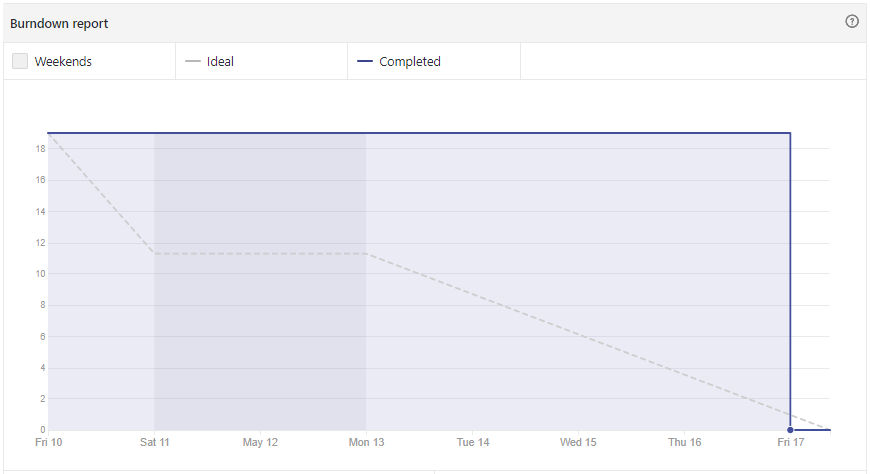
\includegraphics[width=\textwidth]{sprint9}
	\caption{Gráfico del desarrollo del \textit{sprint} 9.}
	\label{fig:sprint9}
\end{figure}

En este \textit{sprint}~\ref{fig:sprint9}, al contrario que en el anterior, no se ha podido realizar todos los objetivos que se tenían, ya que las tareas relacionadas con la creación de la presentación y el guión de Madrid no se han podido hacer.

\subsection{Sprint 10}
 Este \textit{sprint} comenzó el 17 de Mayo de 2019 y terminó el 11 de Junio de 2019.
 
 En este \textit{sprint}, que quería ser el último en el cual hubiese que implementar cosas tanto en las aplicaciones como en el servidor, se quería implementar la descarga del audio en el servidor, cosa que costó mucho, y se quería añadir la parte de clasificación en el servidor con los algoritmos estudiados en los primeros \textit{sprints} y los estudios realizados por el investigador colaborador, Sergio Chico.
 
 La lista resumen de las tareas de este \textit{sprint} es:
 \begin{itemize}
 	\item Desarrollo del paso del audio entre aplicación y servidor con Base64.
 	\item Creación dinámica de nombres en el servidor y eliminación al final de los audios.
 	\item Mejorar la visualización del resultado final.
 	\item Elaboración del método que permite devolver un resultado aleatorio.
 	\item Modificación de los test de la aplicación.
 	\item Corrección de \textit{bugs}.
 	\item Creación de la presentación y el guión para Madrid.
 	\item Presentación del proyecto en Madrid.
 	\item Añadir el sistema de predicción en el servidor.
 	\item Crear e implementar el estándar de errores.
 	\item Refactorización de código.
 	\item Grabación del vídeo en APACE.
 	\item Presentación de la aplicación de interpretación a los cuidadores de APACE.
 \end{itemize}

\begin{figure}
	\centering
	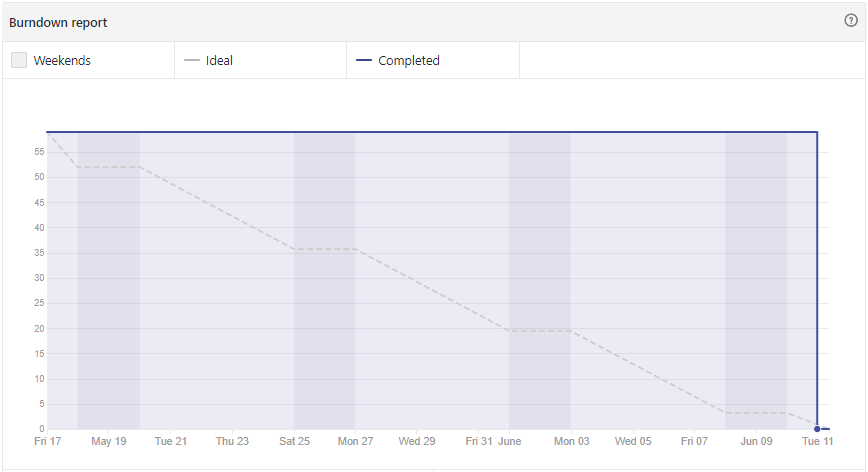
\includegraphics[width=\textwidth]{sprint10}
	\caption{Gráfico del desarrollo del \textit{sprint} 10.}
	\label{fig:sprint10}
\end{figure}

Este \textit{sprint} 10~\ref{fig:sprint10} es sin duda el que más trabajo y problemas ha dado, ya que en el se encuentran varias tareas que han llevado mucho tiempo realizarlas, como por ejemplo la presentación del proyecto en Madrid o el paso del audio al servidor. Aun así, se consiguieron todos los objetivos, sobre todo el objetivo de acabar la implementación de las aplicaciones y del servidor.

\subsection{Sprint 11}
Este \textit{sprint} comenzó el 11 de Junio de 2019 y terminó el 18 de Junio de 2019.

En este \textit{sprint} se pretendía presentar el proyecto ante la prensa y empezar la documentación de la memoria.

Las tareas que se realizaron en el \textit{sprint} fueron:
\begin{itemize}
	\item Presentación del proyecto ante la prensa.
	\item Documentación de la memoria.
\end{itemize}

\begin{figure}
	\centering
	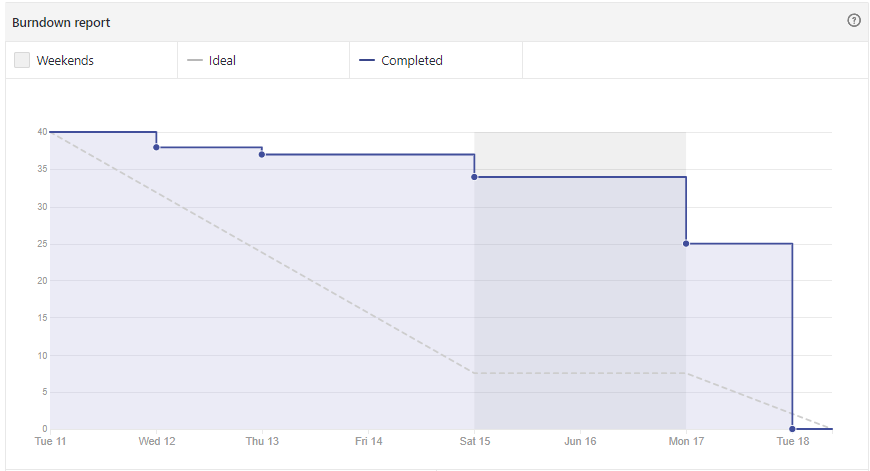
\includegraphics[width=\textwidth]{sprint11}
	\caption{Gráfico del desarrollo del \textit{sprint} 11.}
	\label{fig:sprint11}
\end{figure}

El \textit{sprint} 11~\ref{fig:sprint11} ha sido uno de los más importantes, ya que se ha cumplido, y con creces, uno de los objetivos que se tenían en el proyecto, este objetivo es la difusión mediática. Ya que con la presentación ante la prensa se obtuvo mucha difusión del proyecto.

\subsection{Sprint 12}
ACABAR

Como se puede observar el proyecto, por mi parte, ha tenido más de 400 horas de trabajo de índole muy distinta. Pero cabe destacar que esa no ha sido el único tiempo invertido en el proyecto, sino que hay que añadir el tiempo de investigación de Sergio Chico y el tiempo invertido en todo el proyecto por mis dos tutores, el doctor César Represa y el doctor José Francisco Díez.
\section{Estudio de viabilidad}
En este apartado se quiere comprobar si la realización del proyecto es posible, teniendo en cuenta los aspectos económicos y legales del mismo.
\subsection{Viabilidad económica}
En este subapartado voy a comentar la viabilidad económica del proyecto, en el cual tenemos que calcular tanto los costes de contratación de las 4 personas del equipo de desarrollo, como los gastos en dispositivos, como los gastos para las presentaciones del proyecto.

\subsubsection{Coste de personal}
El personal que ha trabajado en este proyecto es muy variado, y así hay que tenerlo en cuenta en este apartado. Además, hay que tener en cuenta la duración del proyecto que ha ido desde inicio de Diciembre de 2018 hasta principio de Julio de 2019, un total de 7 meses.

Primero empezaremos con los tutores, donde el coste no lo vamos a calcular por la duración del proyecto sino por los créditos impartidos. En primer lugar tenemos al doctor César Represa Pérez, que es profesor colaborador y por otro lado tenemos al doctor José Francisco Díez Pastor. Al no encontrar datos para los profesores colaboradores se han tomado los valores de de doctor.

El sueldo de un doctor en la Universidad de Burgos es de 2360,12 euros al mes~\cite{sueldos}, que daría un total de 28321,44 euros al año. Teniendo en cuenta que un doctor tiene que impartir 32 créditos, aunque luego se suele impartir más, el coste por crédito sería de 28321,44\euro/32 créditos, lo que da un total de 885,04\euro/crédito. Teniendo en cuenta que el Trabajo Fin de Grado es un total de 12 créditos, al ser dos tutores serían 6 créditos por tutor. Lo que darías un coste total por tutor de 5310,27\euro.

Después de calcular el coste de los tutores, paso a calcular el coste de mi compañero investigador y el mio, que van a ser el mismo sueldo por el trabajo de 7 meses. El sueldo mensual neto lo he obtenido del sueldo medio de los empleados en informática~\cite{salario}.

\begin{table}[H]
	\centering
	\begin{tabular}{ll}
		\toprule
		\textbf{Concepto}         & \textbf{Coste}                \\
		\midrule
		Salario mensual neto      & 1575\euro     \\
		Retención IRPF (15\%)     & 428,76\euro   \\
		Seguridad Social (29,9\%)~\cite{gobees} & 854,67\euro   \\
		Salario mensual bruto     & 2858,43\euro  \\
		\midrule
		\textbf{Total 7 meses}    & 20009,01\euro \\		
		\bottomrule
	\end{tabular}
	\caption{Salario trabajador.}
\end{table}

El total de los costes por personal es de:
\begin{table}[H]
	\centering
	\begin{tabular}{ll}
		\toprule
		\textbf{Concepto} & \textbf{Coste} \\ \midrule
		Tutores (x2)      & 10620,54\euro   \\
		Trabajadores (x2) & 40018,02\euro   \\ \midrule
		\textbf{Total}    & 50638,56\euro   \\ \bottomrule
	\end{tabular}
	\caption{Coste de personal.}
\end{table}

\subsubsection{Coste hardware}
En este apartado voy a calcular el coste de los dispositivos hardware que se han usado a lo largo del desarrollo del proyecto junto con su amortización, como la mayoría de los dispositivos hardware, vamos a calcular una armotización de 5 años. En cuanto al coste software no tenemos ningún gasto.

Para el desarrollo he utilizado al menos un dispositivo móvil y dos tablets, y también cuento con la tablet que compraron desde APACE para el proyecto. Además, he usado dos portátiles, pero cuento con el uso de 3 portátiles contando con el ordenador del investigador colaborador.

Las amortizaciones se han calculado por el tiempo usado, es decir, hemos usado todos los dispositivos un total de 7 meses.

\begin{table}[H]
	\centering
	\begin{tabular}{lll}
		\toprule
		\textbf{Concepto}        & \textbf{Coste} & \textbf{Amortización} \\ \midrule
		Dispositivo móvil        & 300\euro        & 35\euro                \\
		Dispositivo tablet (x2)  & 700\euro        & 81,67\euro             \\
		Dispositivo tablet APACE & 350\euro        & 40,83\euro             \\
		Ordenadores (x3)         & 2400\euro       & 280\euro               \\ \midrule
		\textbf{Total}           & 3750\euro       & 437,5\euro             \\ \bottomrule
	\end{tabular}
	\caption{Coste hardware.}
\end{table}

\subsubsection{Otros gastos}
Como ya he comentado, durante el proyecto hemos tenido otro tipo de gastos para realizar las presentaciones, sobre todo en la presentación de Madrid al cual fuimos 3 personas, estos gastos son:

\begin{table}[H]
	\centering
	\begin{tabular}{ll}
		\toprule
		\textbf{Concepto}       & \textbf{Coste} \\ \midrule
		Desplazamiento a Madrid & 40\euro         \\
		Dietas (x3)             & 36\euro         \\ \midrule
		\textbf{Total}          & 76\euro         \\ \bottomrule
	\end{tabular}
	\caption{Coste del viaje a Madrid.}
\end{table}

\subsubsection{Coste Total}
Una vez hemos desglosado todos los costes del proyecto voy a calcular el coste total de este:

\begin{table}[H]
	\centering
	\begin{tabular}{ll}
		\toprule
		\textbf{Concepto} & \textbf{Coste} \\ \midrule
		Coste de personal & 50628,56\euro   \\
		Coste hardware    & 3750\euro       \\
		Otros costes      & 76\euro         \\ \midrule
		\textbf{Total}    & 54454,56\euro   \\ \bottomrule
	\end{tabular}
	\caption{Coste total.}
\end{table}

\subsection{Viabilidad legal}
En este apartado voy a comentar la viabilidad legal de las licencias de las librerías usadas en el proyecto y la licencia final del proyecto.

Desde el comienzo del proyecto le comunicamos tanto a APACE como a Vodafone que necesitábamos saber la licencia que querían, tanto para el transcurso del desarrollo saber que herramientas podíamos usar y obviamente en esta documentación saber que licencia tener. Y aunque se lo preguntásemos en cada una de las reuniones y tras haber enviado varios correos electrónicos a Vodafone, aun no sabemos la licencia que quieren, solo sabemos que quizás sea \textit{open source}. Esto también a afectado al repositorio en \textit{GitHub}, ya que desde un principio lo he tenido que poner en privado, al no saber la licencia del código, pero actualmente lo he modificado a público tras la no respuesta por parte de APACE o Vodafone y por la necesidad de sacar los gráficos del transcurso del desarrollo.

Después de comentar esto, las licencias de las librerías que usamos son:

\begin{table}[H]
	\centering
	\begin{tabular}{ll}
		\toprule
		\textbf{Librería}       & \textbf{Licencia} \\ \hline
		Android Support Library & Apache 2.0        \\
		OpenCSV                 & Apache 2.0        \\
		JavaMail                & GPL v2            \\
		JUnit                   & EPL               \\
		Espresso                & Apache 2.0        \\
		Flask                   & BSD 3 New              \\
		Pandas                  & BSD 3 New            \\
		Numpy                   & BSD 3 New           \\
		Scikit-Learn            & BSD 3 New   \\
		Matplotlib              & PSFL              \\ \bottomrule
	\end{tabular}
	\caption{Licencias de las librerías.}
\end{table}

Además, hemos usado los pictogramas de la pagina de \textit{ARASAAC}~\cite{arasaac}, que tiene un licencia CC BY-NC-SA 3.0 ES. Por lo que las imágenes que he tenido que modificar tienen esta misma licencia.

El uso de una licencia EPL, que nos obligaría a descargar las librerías con esta licencia en tiempo de ejecución, ya que no nos permite distribuirlas. Pero, en nuestro caso, la única librería que usa la licencia EPL es \textit{JUnit}, una de las librerías que se usan para probar el código. Como esta no se distribuye junto con el código, no nos obliga a descargarla en tiempo de ejecución.

Tras comprobar las licencias de las librerías que usamos en el proyecto, y ante la negativa de APACE o Vodafone de darnos una respuesta a la pregunta de qué licencia usar, he decidido que la licencia del proyecto sea GPL v3, ya que es la licencia más restrictiva de las herramientas que tengo y me permite en un futuro patentar el software creado.